\documentclass[12pt, a4paper]{article}

\usepackage{array}
\usepackage[portuguese]{babel}
\usepackage{chngpage}
\usepackage{enumitem}
\usepackage{float}
\usepackage[a4paper, margin=2cm]{geometry}
\usepackage{graphicx}
\usepackage{hyperref}
\usepackage{longtable}
\usepackage{lscape}
\usepackage{pdfpages}
\usepackage{setspace}

\makeatletter
\renewcommand\section[1]{
    \newpage
    \thispagestyle{empty}
    \vspace*{\fill}
    \@startsection{section}{1}{\z@}{0px}{50px}{\normalfont\Huge\bfseries}{#1}
    \vspace*{\fill}
    \newpage
}
\makeatother

\title{\textbf{Desenvolvimento de Sistemas de Software \\ \large Trabalho Prático -- Fase I}}
\date{19 de outubro 2024}
\author{
    Grupo 13 \\
    \url{https://github.com/LEI-DSS/DSS2425-Grupo-13}
}

\begin{document}

\begin{center}
    
\includegraphics[width=0.25\textwidth]{Imagens/Capa/EE-C.eps}
\end{center}

{\let\newpage\relax\maketitle}
\maketitle
\thispagestyle{empty}

\chardef\_=`_
\onehalfspacing
\setlength{\parskip}{\baselineskip}
\setlength{\parindent}{0pt}
\def\arraystretch{1.5}

\vspace{2cm}
\begin{center}
    \begin{tabular}{>{\centering}p{0.25\textwidth}
                    >{\centering}p{0.25\textwidth}
                    >{\centering\arraybackslash}p{0.25\textwidth}}
        
\includegraphics[width=3.5cm]{Imagens/Capa/A104188.png} &
        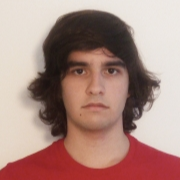
\includegraphics[width=3.5cm]{Imagens/Capa/A104348.png} &
        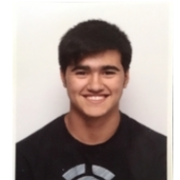
\includegraphics[width=3.5cm]{Imagens/Capa/A95748.png}  \\

        Ana Carolina & Humberto Gomes & João Torres \\
        A104188      & A104348        & A95748
    \end{tabular}

    \begin{tabular}{>{\centering}p{0.25\textwidth}
                    >{\centering\arraybackslash}p{0.25\textwidth}}
        
\includegraphics[width=3.5cm]{Imagens/Capa/A104541.png} &
        
\includegraphics[width=3.5cm]{Imagens/Capa/A100612.png} \\

        José Lopes & José Matos \\
        A104541    & A100612
    \end{tabular}
\end{center}

\section{Modelo de Domínio}

\section{Casos de Uso}

\section{Anexos}

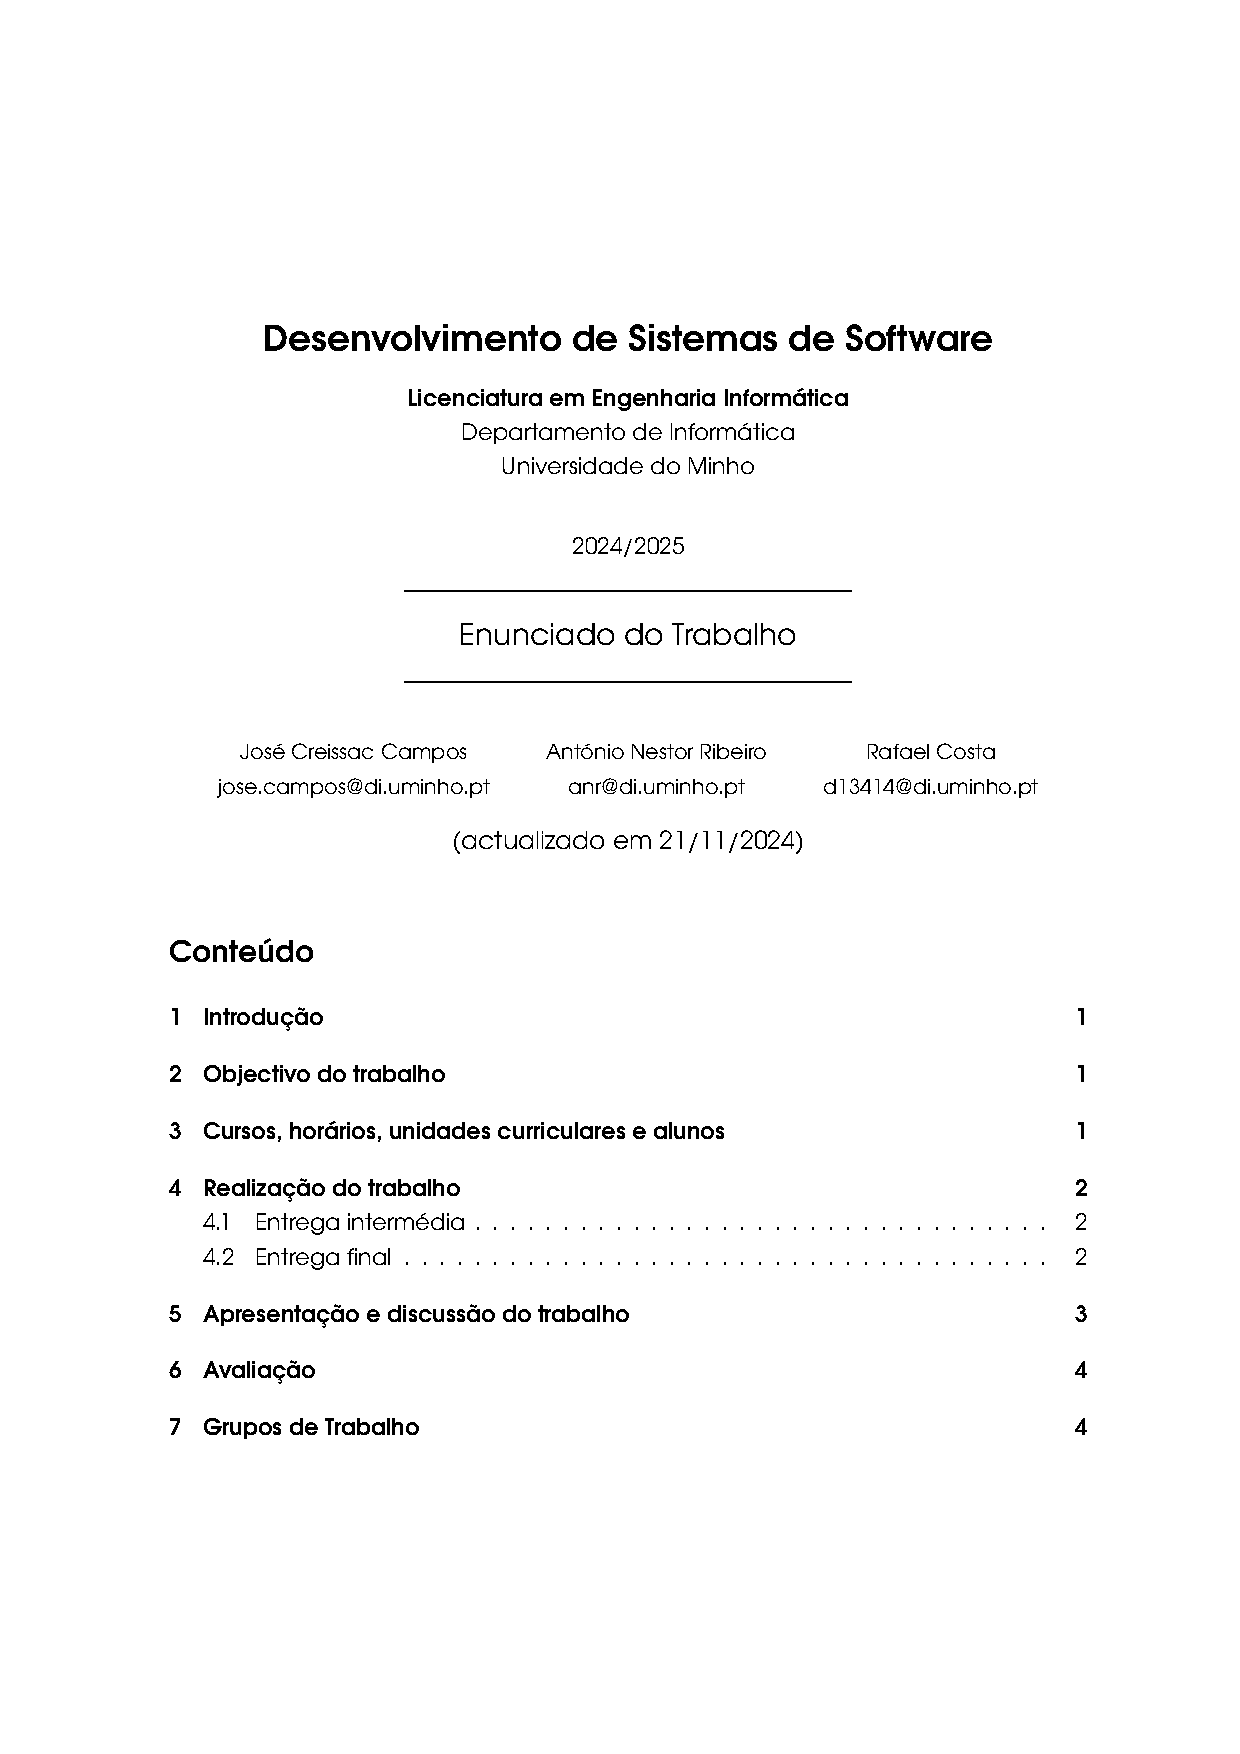
\includepdf[pages=1,pagecommand=\subsection{Enunciado do Trabalho}\thispagestyle{empty}]
    {../Enunciado.pdf}
\includepdf[pages=2-]{../Enunciado.pdf}

\subsection{Cenários}
\label{use-cases}

\textbf{O Diretor de Curso}

Após ter obtido a lista de alunos inscritos às UC do curso, através da Intranet, o diretor de curso
acedeu à aplicação de gestão de turnos e, depois de se ter autenticado, importou a lista de alunos
para o sistema. Como já anteriormente tinha importado a lista de UC e os seus horários, ficou em
condições de iniciar a geração dos horários dos alunos. Antes de o fazer, no entanto, definiu as
preferências que tinha recebidos dos docentes de algumas UC.

Uma das UC pediu que os alunos repetentes fossem colocados em turnos distintos dos alunos de
primeira inscrição para poder aplicar um método de ensino diferenciado. Uma outra enviou os grupos
de trabalho e pediu que os elementos de cada grupo ficassem no mesmo turno PL. Ainda uma outra,
pediu que os alunos fossem distribuídos pelos turnos de modo que ficassem agrupados por proximidade
da média de curso (uma forma de procurar ter turmas mais homogéneas). Finalmente, várias UC
definiram tamanhos máximos para os turnos TP/PL, diferentes do valor por omissão usado no curso.

Após configurar as preferências das UC, o diretor de curso pediu ao sistema uma primeira alocação
dos alunos aos turnos. O sistema realizou essa alocação, mas foi incapaz de colocar 45 alunos, por
não conseguir respeitar todas as preferências sem evitar conflitos nos seus horários.

O diretor de curso procedeu então à alocação manual desses alunos aos turnos disponíveis. Em alguns
casos o sistema avisou-o de conflitos nos horários dos alunos (ou no cumprimento das preferências
das UC). Na impossibilidade de evitar alguns desses conflitos, o diretor de curso optou por dar
prioridade aos alunos de primeira inscrição, fazendo a distribuição manual de modo a evitar
conflitos a esses alunos.

Após terminar a distribuição, o diretor de curso publicou os horários dos alunos.

\textbf{Os alunos}

A Maria recebeu uma notificação por email de que o seu horário tinha sido publicado. Acedeu à sua
versão da aplicação de gestão de turnos, consultou o horário e aproveitou para o exportar para a
sua agenda.

\end{document}
